% Template LaTeX file for DAFx-19 papers
%
% To generate the correct references using BibTeX, run
%     latex, bibtex, latex, latex
% modified...
% - from DAFx-00 to DAFx-02 by Florian Keiler, 2002-07-08
% - from DAFx-02 to DAFx-03 by Gianpaolo Evangelista
% - from DAFx-05 to DAFx-06 by Vincent Verfaille, 2006-02-05
% - from DAFx-06 to DAFx-07 by Vincent Verfaille, 2007-01-05
%                          and Sylvain Marchand, 2007-01-31
% - from DAFx-07 to DAFx-08 by Henri Penttinen, 2007-12-12
%                          and Jyri Pakarinen 2008-01-28
% - from DAFx-08 to DAFx-09 by Giorgio Prandi, Fabio Antonacci 2008-10-03
% - from DAFx-09 to DAFx-10 by Hannes Pomberger 2010-02-01
% - from DAFx-10 to DAFx-12 by Jez Wells 2011
% - from DAFx-12 to DAFx-14 by Sascha Disch 2013
% - from DAFx-15 to DAFx-16 by Pavel Rajmic 2015
% - from DAFx-16 to DAFx-17 by Brian Hamilton 2016
% - from DAFx-18 to DAFx-19 by Dave Moffat 2019
%
% Template with hyper-references (links) active after conversion to pdf
% (with the distiller) or if compiled with pdflatex.
%
% 20060205: added package 'hypcap' to correct hyperlinks to figures and tables
%                      use of \papertitle and \paperauthorA, etc for same title in PDF and Metadata
% 05/02/2019: Package 'hypcap' removed, and replaced with 'caption', to allow for the inclusion
%			of a CC UP licence.
%
% 1) Please compile using latex or pdflatex.
% 2) If using pdflatex, you need your figures in a file format other than eps! e.g. png or jpg is working
% 3) Please use "paperftitle" and "pdfauthor" definitions below

%------------------------------------------------------------------------------------------
%  !  !  !  !  !  !  !  !  !  !  !  ! user defined variables  !  !  !  !  !  !  !  !  !  !  !  !  !  !
% Please use these commands to define title and author(s) of the paper:
\def\papertitle{Real-Time Implementation of the Elasto-Plastic Bow Model applied to Finite-Difference Schemes}
\def\paperauthorA{Silvin Willemsen}
\def\paperauthorB{Stefania Serafin}
\def\paperauthorC{Stefan Bilbao}

% Authors' affiliations have to be set below

%------------------------------------------------------------------------------------------
\documentclass[twoside,a4paper]{article}
% \usepackage{tikz}
% \tikzset{>=latex}
% \tikzstyle{block} = [draw,minimum size=0.5cm]
% \usetikzlibrary{math}
\usepackage{dafx_19}
\usepackage{amsmath,amssymb,amsfonts,amsthm}
\usepackage{euscript}
\usepackage[latin1]{inputenc}
\usepackage[T1]{fontenc}
\usepackage{ifpdf}
\usepackage{scalerel}

\usepackage[english]{babel}
\usepackage{caption}
\usepackage{subfig} % or can use subcaption package
\usepackage{color}
\newenvironment{rcases}
  {\left.\begin{alignedat}{2}}
  {\end{alignedat}\right\rbrace}
\DeclareMathOperator{\sgn}{sgn}
\setcounter{page}{1}
\ninept

\usepackage{times}
% Saves a lot of ouptut space in PDF... after conversion with the distiller
% Delete if you cannot get PS fonts working on your system.

% pdf-tex settings: detect automatically if run by latex or pdflatex
\newif\ifpdf
\ifx\pdfoutput\relax
\else
   \ifcase\pdfoutput
      \pdffalse
   \else
      \pdftrue
\fi

\ifpdf % compiling with pdflatex
  \usepackage[pdftex,
    pdftitle={\papertitle},
    pdfauthor={\paperauthorA, \paperauthorB},
    colorlinks=false, % links are activated as colror boxes instead of color text
    bookmarksnumbered, % use section numbers with bookmarks
    pdfstartview=XYZ % start with zoom=100% instead of full screen; especially useful if working with a big screen :-)
  ]{hyperref}
  \pdfcompresslevel=9
%   \usepackage[pdftex]{graphicx}
%  \usepackage[figure,table,hypcap=true]{caption}
\else % compiling with latex
  
  \usepackage[dvips]{epsfig,graphicx}
  \usepackage[dvips,
    colorlinks=false, % no color links
    bookmarksnumbered, % use section numbers with bookmarks
    pdfstartview=XYZ % start with zoom=100% instead of full screen
  ]{hyperref}
  % hyperrefs are active in the pdf file after conversion
%  \usepackage[figure,table,hypcap=true]{caption}
\fi
  \usepackage[hypcap=true]{caption}
\title{\papertitle}

%-------------SINGLE-AUTHOR HEADER STARTS (uncomment below if your paper has a single author)-----------------------
%\affiliation{
%\paperauthorA \,\sthanks{This work was supported by the XYZ Foundation}}
%{\href{http://dafx2019.bcu.ac.uk/}{Digital Media Technology Lab} \\ Birmingham City University \\ Birmingham, UK \\ {\tt \href{mailto:dafx2019@gmail.com}{dafx2019@gmail.com}}}
%-----------------------------------SINGLE-AUTHOR HEADER ENDS------------------------------------------------------

%---------------TWO-AUTHOR HEADER STARTS (uncomment below if your paper has two authors)-----------------------
\twoaffiliations{
\paperauthorA, \paperauthorB}
{{Multisensory Experience Lab, CREATE,} \\ Aalborg University Copenhagen\\
  Copenhagen, Denmark\\ {\tt \href{mailto:sil@create.aau.dk}{\{sil, sts\}@create.aau.dk}}}
{\paperauthorC}
{ Acoustics and Audio Group \\ University of Edinburgh\\
    Edinburgh, UK\\
     {\tt \href{mailto:s.bilbao@ed.ac.uk}{s.bilbao@ed.ac.uk}}}
%-------------------------------------TWO-AUTHOR HEADER ENDS------------------------------------------------------

%---------------THREE-AUTHOR HEADER STARTS (uncomment below if your paper has three authors)-----------------------
% \threeaffiliations{
% \paperauthorA \,\sthanks{This work was supported by the XYZ Foundation}}
% {\href{http://dafx2019.bcu.ac.uk/}{Digital Media Technology Lab} \\ Birmingham City University \\ Birmingham, UK \\ {\tt \href{mailto:dafx2019@gmail.com}{dafx2019@gmail.com}}}
% {\paperauthorB \,\sthanks{Thanks to the predecessors for the templates}}
% {\href{http://dafx2018.web.ua.pt/}{IEETA} \\ University of Aveiro \\ Aveiro, Portugal \\ {\tt \href{mailto:dafx2018_papers@ua.pt}{dafx2018\_papers@ua.pt}}}
% {\paperauthorC \,\sthanks{Illustrious contributor}}
% {\href{http://www.acoustics.ed.ac.uk}{Acoustics and Audio Group,} \\ University of Edinburgh\\ Edinburgh, UK\\ {\tt \href{mailto:dafx17@ed.ac.uk}{dafx17@ed.ac.uk}}}
%-------------------------------------THREE-AUTHOR HEADER ENDS------------------------------------------------------

%----------------FOUR-AUTHOR HEADER STARTS (uncomment below if your paper has four authors)-----------------------
% \fouraffiliations{
% \paperauthorA \,\sthanks{This work was supported by the XYZ Foundation}}
% {\href{http://dafx2019.bcu.ac.uk/}{Digital Media Technology Lab} \\ Birmingham City University \\ Birmingham, UK \\ {\tt \href{mailto:dafx2019@gmail.com}{dafx2019@gmail.com}}}
% {\paperauthorB \,\sthanks{Thanks to the predecessors for the templates}}
% {\href{http://dafx2018.web.ua.pt/}{IEETA} \\ University of Aveiro \\ Aveiro, Portugal \\ {\tt \href{mailto:dafx2018_papers@ua.pt}{dafx2018\_papers@ua.pt}}}
% {\paperauthorC \,\sthanks{Illustrious contributor}}
% {\href{http://www.acoustics.ed.ac.uk}{Acoustics and Audio Group,} \\ University of Edinburgh\\ Edinburgh, UK\\ {\tt \href{mailto:dafx17@ed.ac.uk}{dafx17@ed.ac.uk}}}
% {\paperauthorD \,\sthanks{This guy is a very good fellow}}
% {\href{http://dafx16.vutbr.cz}{SPLab} \\ Brno University of Technology \\ Brno, Czech Republic \\ {\tt \href{mailto:dafx16@vutbr.cz}{dafx16@vutbr.cz}}}
%-------------------------------------FOUR-AUTHOR HEADER ENDS------------------------------------------------------

\usepackage[dvipsnames]{xcolor}
\def\SBcomment[#1]{\textcolor{Red}{#1}}
\def\SWcomment[#1]{\textcolor{Blue}{#1}}

\begin{document}
% more pdf-tex settings:
\ifpdf % used graphic file format for pdflatex
  \DeclareGraphicsExtensions{.png,.jpg,.pdf, .eps} 
\else  % used graphic file format for latex
  \DeclareGraphicsExtensions{.eps}
\fi

\maketitle

\begin{abstract}
This paper describes the a real-time implementation of the elasto-plastic friction model applied to a stiff string implemented using finite-difference schemes (FDSs). 
\end{abstract}

\section{Introduction}
\label{sec:intro}
In the field of physical modelling for sound synthesis, the implementation of the bowed string is a challenging endeavour. This is mainly due to the non-linear relationship between the bow and the string, the friction. Friction models that describe this relationship can be subdivided into static and dynamic models, the latter of which has only seen major developments in the last two decades. As opposed to static friction models, dynamic models describe the friction force through a differential equations and exhibit hysteresis loops in the force vs. velocity plane.

Most friction models are calculated as a function of the relative velocity between the bow and the string only. In \cite{Woodhouse2003}, Woodhouse proposed a thermal friction model that added the temperature of the rosin as an extra dependency for the friction force. A more general model is the elasto-plastic model, as first proposed in \cite{Dupont2002} by Dupont et al. It assumes that the friction between the bow and the string is caused by a large quantity of bristles, each of which contributes to the total amount of friction. The bristle deflection is used as an extra independent variable for calculating the friction force. Still today, the elasto-plastic model is considered one of the most accurate friction models [source]. 

The first simulations of different non-linear oscillators, including bowed strings, were presented by McIntyre, et al. in \cite{McIntyre1983}. Based on this, Smith published the first real-time implementation of the bowed string using digital waveguides for the string and a look-up table for the friction model in \cite{Smith1986}. Simultaneously, Florens, et al. published a real-time implementation using mass-spring systems for the string and a static friction model for the bow in \cite{Florens1986}.

Partial differential equations are well known to mathematically and accurately describe the behaviour of musical instruments. Considered to approximate these equations most accurately (especially in the case of non-linear systems) are finite-difference time-domain (FDTD) methods \cite{Bilbao2009, Bilbao2018}. In \cite{Maestre2014} the authors adapted the aforementioned thermal model to work in real-time using digital waveguides (DW) for the string implementation and a combination of DW and FDTD methods for the bowing interaction. In \cite{Desvages2017}, Desvages used FDTD methods for the implementation of the string and the static double exponential friction model introduced in \cite{Smith2000}, which was, however, not implemented in real-time. To the best of the authors' knowledge, the only known real-time implementation of any bow model applied to to FDTD strings was presented in \cite{Willemsen2019} where the soft exponential friction function presented in \cite{Bilbao2009} was used. The current work can be considered an extension on this.

We are interested to bridge the gap between highly accurate physical models and efficient implementation so that these models can be played in real-time. In this work, we present an implementation of the elasto-plastic friction model applied as an external force to a finite-difference implementation of the damped stiff string. Furthermore, we show that it is possible to play the string in real-time using the Sensel Morph controller \cite{Sensel2019}.

This paper is structured as follows: Section \ref{sec:stiffString} describes the PDE of the stiff damped string, Section \ref{sec:elasto} explains the elasto-plastic bow model and Section \ref{sec:discretisation} explains how these models are discretised using finite-difference schemes. Section \ref{sec:implementation} then elaborates on the implementation and Section \ref{sec:results} shows the computational results of this. Finally \ref{sec:conclusion} concludes.

\section{Stiff String}\label{sec:stiffString}
Using the subscripts $t$ and $x$ to denote a single derivative with respect to time and space respectively, the partial differential equation of the damped stiff string is defined as \cite{Bilbao2009}
\begin{equation}\label{eq:PDE}
    u_{tt} = c^2u_{xx}-\kappa^2u_{xxxx}-2\sigma_0u_t+2\sigma_1u_{txx},
\end{equation}
where $c = \sqrt{T/\rho A}$ is the wave speed (in m/s) with tension $T$ (in N), material density $\rho$ (in kg$\cdot$m$^{-3}$) and cross-sectional area $A$ (in m$^2$), $\kappa = \sqrt{EI/\rho A}$ is the stiffness coefficient (in m$^2$/s) with Young's Modulus $E$ (in Pa) and area moment of inertia $I$ (in m$^4$) and frequency independent and frequency dependent damping coefficients $\sigma_0 \geq 0$ and $\sigma_1 \geq 0$.

In our implementation we assume simply supported boundary conditions, which, for a string of length $L$, are defined as
\begin{equation}
    u = u_{xx} = 0 \quad \text{where} \quad x = 0, L.
\end{equation}

\section{Elasto-Plastic Bow Model}\label{sec:elasto}
% \begin{figure}[h]
%     \centering
%     \begin{tikzpicture}
    
%     \def\radius{6}; % Radius of the string (>2!)
%     \pgfmathsetmacro{\reps}{3}; % How may back-and-forths in the drawing of the springs
%     \def\horShift{0.5}; %how far the bow is shifted to the right in b)
%     \def\bowSpacing{0.2};
%     \def\drawingSpacing{1.5}
%     \def\bowWidth{5};
    
%     %subfigure letters
%     \node (A) at (-2.8, 0.5) {a)};
%     \node (B) at (-2.8, 0.5 - \drawingSpacing) {b)};
%     \node (C) at (-2.8, 0.5 - \drawingSpacing * 2) {c)};
%     \node (D) at (-2.8, 0.5 - \drawingSpacing * 3) {d)};
    
%     %bow velocity arrow
%     \draw[->] (-1, 1.3) -- (1, 1.3) node [midway, above] (velText) {$v_\text{B}$};
    
%     \pgfmathsetmacro{\zCoordTop}{0};
%     \pgfmathsetmacro{\zYCoordBottom}{0};
%     \def\springForZ{2}
%     \foreach \drawing in {0, ..., 3}
%     {
%         %% Draw String
%         \begin{scope}
%             \clip (-1.5,-0.2- \drawing * \drawingSpacing) rectangle (1.5,1.5);
%             \draw (0,-\radius + 0.25 - \drawing * \drawingSpacing) circle(\radius);
%         \end{scope}

%         %% Draw Bow
%         \def\halfBW{\bowWidth*0.5}
%         \pgfmathsetmacro{\halfNumDiag}{0.5 * \bowWidth / \bowSpacing};
%         \draw[-] (-\halfBW + \drawing * \horShift,1 - \drawing * \drawingSpacing) -- (\halfBW + \drawing * \horShift, 1 - \drawing * \drawingSpacing);
%         \foreach \bowDiag in {-\halfNumDiag, ...,\halfNumDiag}
%         {
%         \pgfmathtruncatemacro{\bD}{\bowDiag}
%         % \ifnum\drawing=0
%         %     \ifnum\bD<-1
%         %         \draw[-] (\drawing * \horShift + \bowDiag * \bowSpacing, -\drawing * \drawingSpacing + 1) -- (\drawing * \horShift + \bowDiag * \bowSpacing + 0.1, -\drawing * \drawingSpacing + 0.1 + 1);
%         %         \else
%         %         \ifnum\bD>1
%         %             \draw[-] (\drawing * \horShift + \bowDiag * \bowSpacing, -\drawing * \drawingSpacing + 1) -- (\drawing * \horShift + \bowDiag * \bowSpacing + 0.1, \drawing * -2 + 0.1 + 1);
%         %         \fi
%         %     \fi
%         % \else
%             \draw[-] (\drawing * \horShift + \bowDiag * \bowSpacing, -\drawing * \drawingSpacing + 1) -- (\drawing * \horShift + \bowDiag * \bowSpacing + 0.1, -\drawing * \drawingSpacing + 0.1 + 1);
%         % \fi
            
%         }
        
%         \def\brokenSprings{{0, 1, 1, 0, 1, 0}};
%         %% Draw Springs
%         \foreach \springNo in {0, ..., 5}
%         {
%             % Calculate spring length depending on the radius of the string
%             \pgfmathsetmacro{\startX}{\springNo  * 0.5 - 1.25};
%             \pgfmathsetmacro{\calcSpace}{(\radius + 1) - \radius * sin(acos(\startX/\radius)) - 0.25};
%             \pgfmathsetmacro{\springLength}{sqrt(\calcSpace*\calcSpace+\drawing*\horShift*\drawing*\horShift)};
            
%             \pgfmathsetmacro{\spacing}{\springLength / (\reps + 2)}; 
%             % spacing between two spring-back-and-forths
%             \ifnum\drawing=0
%                 \pgfmathsetmacro{\rot}{0};
%             \else
%                 \pgfmathsetmacro{\rot}{(270+(atan(\calcSpace/(\drawing*\horShift))))}; %rotation of the springs
%             \fi
            
%             \ifnum\drawing=1
%                 \ifnum\springNo=\springForZ
%                     \pgfmathsetmacro{\resTwo}{sqrt(\springLength*\springLength-\horShift*\horShift)};
%                     \global\let\zCoordBottom = \resTwo;
%                 \fi
%             \fi
        
%             \pgfmathsetmacro{\isBroken}{\brokenSprings[\springNo]};
%             % debug code
%             % \node (nodeTest\springNo) at (\springNo*1.1-2, -3 - 1 * \drawing + 0.3 * \springNo) {\isBroken};
            
%             \begin{scope}[shift={(\startX + \drawing * \horShift,1 -\drawing * \drawingSpacing)}]
%                 \pgfmathsetmacro{\xWidth}{0.1 - (\drawing * 0.02)};
%                 \draw[-, rotate = \rot] (0, 0) -- (0, -\spacing * 0.5);
%                 \draw[-, rotate = \rot] (0, -\spacing * 0.5) -- (\xWidth, -\spacing);
%                 \def\Y{-\spacing}
%                 \foreach \idx in {1,...,\reps}
%                 {
%                     \pgfmathsetmacro{\idxMinOne}{\idx-1};
%                     \ifnum\drawing=2
%                         \ifnum\isBroken=1
%                             \pgfmathtruncatemacro{\idxT}{\reps * 0.5 + 1}
%                             \ifnum\idx=\idxT
%                                 \draw[-, rotate = \rot] (\xWidth, \Y - \idxMinOne * \spacing) -- (-\xWidth,\Y - \idx * \spacing*0.6);
%                                 \draw[-, rotate = \rot] (\xWidth, \Y - \idxMinOne * \spacing * 1.66) -- (-\xWidth,\Y - \idx * \spacing);
%                             \else
%                                 \draw[-, rotate = \rot] (\xWidth, \Y - \idxMinOne * \spacing) -- (-\xWidth,\Y - \idx * \spacing);
%                             \fi
%                         \else
%                                 \draw[-, rotate = \rot] (\xWidth, \Y - \idxMinOne * \spacing) -- (-\xWidth,\Y - \idx * \spacing);
%                         \fi
%                     \else
%                         \ifnum\drawing=3
%                             \pgfmathtruncatemacro{\idxT}{\reps * 0.5 + 1}
%                             \ifnum\idx=\idxT
%                                 \draw[-, rotate = \rot] (\xWidth, \Y - \idxMinOne * \spacing) -- (-\xWidth,\Y - \idx * \spacing*0.6);
%                                 \draw[-, rotate = \rot] (\xWidth, \Y - \idxMinOne * \spacing * 1.66) -- (-\xWidth,\Y - \idx * \spacing);
%                             \else
%                                 \draw[-, rotate = \rot] (\xWidth, \Y - \idxMinOne * \spacing) -- (-\xWidth,\Y - \idx * \spacing);
%                             \fi
%                         \else
%                             \draw[-, rotate = \rot] (\xWidth, \Y - \idxMinOne * \spacing) -- (-\xWidth,\Y - \idx * \spacing);
%                         \fi
%                     \fi
%                     \pgfmathsetmacro{\invXWidth}{\xWidth*-1};
%                     \global\let\xWidth = \invXWidth;
%                     \pgfmathsetmacro{\lastYPre}{\Y - \idx * \spacing};
%                     \global\let\lastY = \lastYPre;
%                 }
%                 \draw[-, rotate = \rot] (\xWidth, \lastY) -- (0, \lastY - \spacing * 0.5);
%                 \draw[-, rotate = \rot] (0, \lastY - \spacing * 0.5) -- (0, \lastY - \spacing);
%              \end{scope}
             
%         }
%         % \draw[<->] (2,2-0.707) -- node[right] {$r=\sqrt{2} \Rightarrow A=\pi(\sqrt{2})^2=2\pi$} (2,2+0.707);
        
%         % \node(stringText) at (0, -\drawing * 2) {string};
%         % \node[block, minimum height = 0.15cm, fill=white, draw=white] (bowText) at (\drawing * \horShift, 1.23 - \drawing * 2) {bow};
%     }
%     \filldraw[black] (-1.25+\springForZ*0.5 + \horShift,1-\drawingSpacing) circle (1pt) node[anchor=center](topZ){};
%     \filldraw[black] (-1.25++\springForZ*0.5,1-\zCoordBottom-\drawingSpacing) circle (1pt) node[anchor=center](bottomZ){};
    
%     \node [](leftNode) at (-1.25+\springForZ*0.5,-\drawingSpacing - 0.1) {};
%     \node [](rightNode) at (-1.25 +\springForZ*0.5 + \horShift,-\drawingSpacing - 0.1) {};
    
%     \draw[<->] (leftNode.center) -- (rightNode.center) node [midway, above] (TextNode) {$z$};
%     \draw[dashed, darkgray] (leftNode) -- (bottomZ);
%     \draw[dashed, darkgray] (rightNode) -- (topZ);
%     %% Draw bow and string texts
%         \node(stringText) at (0, 0) {string};
%         \node(bowText) at (3, 1.1) {bow};
%     %% Draw descriptions of z
%     \def\zTexts{{"$z=0$", "$0<|z|<z_{\text{ba}}$", "$z_{\text{ba}}<|z|< z_\text{ss}$", "$|z|>z_\text{ss}$"}};
    
%     \node[anchor = east](zText1) at (5.3, 0.5) {$z=0$};
%     \node[anchor = east](zText1) at (5.3, 0.5 - \drawingSpacing) {$0<|z|\leq z_{\text{ba}}$};
%     \node[anchor = east](zText1) at (5.3, 0.5 - \drawingSpacing * 2) {$z_{\text{ba}}<|z|\leq |z_\text{ss}|$};
%     \node[anchor = east](zText1) at (5.3, 0.5 - \drawingSpacing * 3) {$|z|>|z_\text{ss}|$};
    
%     \end{tikzpicture}
%     \caption{\it Microscopic displacements of the bristles between the bow and the string. The bow moves right with a velocity of $v_\text{B}$. a) The initial state is where the average bristle displacement $z=0$. b) The bow has moved right relative to the string. The purely elastic, or presliding regime is entered (stick). c) After the break-away displacement $z_\text{ba}$, more and more bristles start to `break'. This is defined as the elasto-plastic regime. d) After all bristles have `broken', the steady state (slip) is reached and the purely plastic regime is entered.}
%     \label{fig:elastoPlastic}
% \end{figure}

As mentioned, the elasto-plastic bow model assumes that the friction between the bow and the string is caused by a large quantity of bristles, each of which contributes to the total amount of friction. See Figure \ref{fig:elastoPlastic} for a visual explanation of this. The bristles are assumed to be stiff springs with damping and can `break' after a given break-away displacement. An extra term can be added to \eqref{eq:PDE} to include the bowing interaction
\begin{equation}
    \begin{aligned}
    \label{eq:bowingTerm}
        u_{tt} = \hdots - \delta(x-x_\text{B})f(v, z)/\rho A,
    \end{aligned}
\end{equation}

\SWcomment[Alright, I guess this works now :) ] with spatial Dirac delta function $\delta(x-x_\text{B})$ applying the bowing function $f$ at bowing position $x_\text{B}$. The bowing function is dependent on the relative velocity between the string at the bowing point and the bow
\begin{equation}\label{eq:relVel}
  v = u_t(x_\text{B}) - v_\text{B}
\end{equation}
and the aforementioned average bristle displacement $z$. In the following we will use the definitions found in \cite{Dupont2002}. The bowing function itself is defined as:
\begin{equation}\label{eq:forceFunction}
    f(v, z) = s_0z + s_1\dot z + s_2v
\end{equation}
where $s_0$ is the bristle stiffness (in N/m), $s_1$ is the damping coefficient (in N$\cdot$ s/m) and $s_2$ is the viscous friction (in N$\cdot$ s/m).
Moreover, the rate of change of $z$ is related to $v$ through
\begin{equation}\label{eq:zdot}
    \dot z(v, z) = v \bigg[ 1-  \alpha(v, z)\frac{z}{z_\text{ss}(v)}\bigg ]
\end{equation}
where $\dot{z}$ indicates an ordinary time derivative of $$$z_\text{ss}$ is the steady-state function
\begin{equation}
    z_\text{ss}(v) = \frac{\sgn(v)}{s_0}\Big[f_\text{c}+(f_\text{s}-f_\text{c})e^{-(v/v_\text{s})^2}\Big].
\end{equation}
with Stribeck velocity $v_\text{s}$ (in m/s), coulomb force $f_\text{c} = f_\text{N}\mu_\text{c}$ and stiction force $f_\text{s} = f_\text{N}\mu_\text{s}$ (both in N). Here $f_\text{N}$ is the normal force (in N) and $\mu_\text{c}$ and $\mu_\text{s}$ are the dynamic and static friction coefficient respectively. 
Furthermore, the adhesion map between the bow and the string is defined as
\begin{equation}\label{eq:adhesionMap}
\alpha(v, z) 
\begin{aligned}
    \begin{cases}
    \begin{rcases}
        &0 & |z| \leq z_\text{ba}\\
       &\alpha_\text{m}(v,z)&\ \, z_\text{ba}<|z|\leq|z_\text{ss}(v)|\\        &1 &|z|>|z_\text{ss}(v)|
        \end{rcases} 
        
        &\!\!\!\!\!\text{if}\  \sgn(v)=\sgn(z)\\
        \,0&\!\!\!\!\!\text{if}\  \sgn(v)\neq\sgn(z),
    \end{cases}
    \end{aligned}
\end{equation}
where the transition between the elastic and plastic behaviour is defined as
\begin{equation}\label{eq:alphaM}
    \alpha_\text{m} = \frac{1}{2}\bigg[1+\sgn(z)\sin\bigg(\pi\frac{z-\sgn(z)\frac{1}{2}(|z_\text{ss}(v)|+z_\text{ba})}{|z_\text{ss}(v)|-z_\text{ba}}\bigg)\bigg],
\end{equation}
with break-away displacement $z_\text{ba}$, i.e. where the bristles start to break, as mentioned at the beginning of this section. A visualisation of the adhesion map can be found in Figure \ref{fig:alphaPlot}. 

Interesting to note is that in the literature on this topic, several errors can be found in the definition of $\alpha(v,z)$: 1) all uses of $z_\text{ss}$ in \eqref{eq:adhesionMap} and \eqref{eq:alphaM} lack the absolute value operator, 2) the multiplications with $\sgn(z)$ in \eqref{eq:alphaM} are excluded, 3) $\alpha(v,z)$ is undefined for $|z|=z_\text{ba}$ and $|z|=|z_\text{ss}(v)|$. It can be shown that only with the definitions presented here, is it possible to obtain the curve shown in Figure \ref{fig:alphaPlot}. \textbf{<- maybe this paragraph is a little too pretentious haha}

\begin{figure}[ht]
\centerline{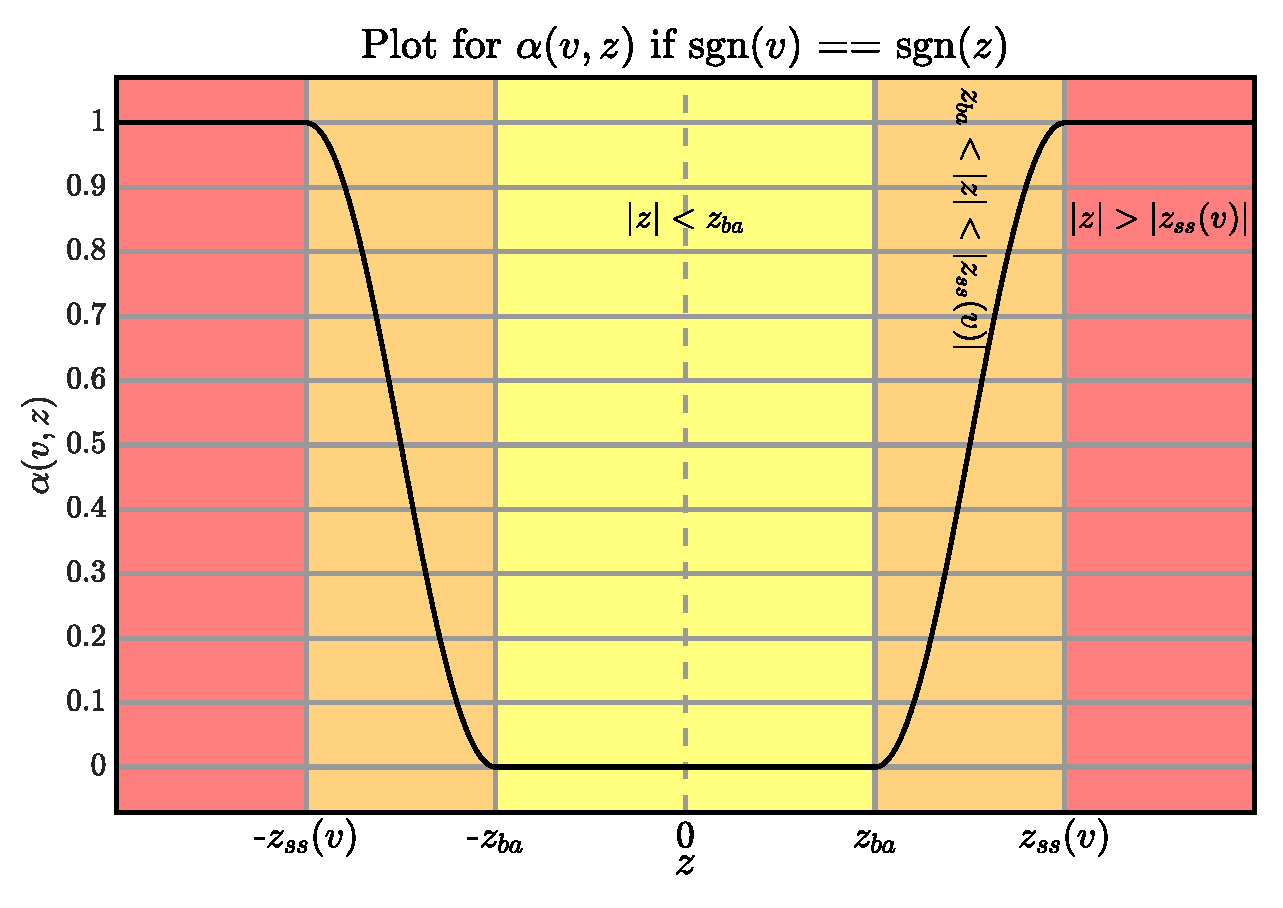
\includegraphics[width=1.0\columnwidth]{untitled.eps}}
\caption{\label{fig:alphaPlot}{\it A plot of the adhesion map $\alpha(v,z)$ plotted against $z$ when the signs of $v$ and $z$ are the same. The different regions of the map are shown with the coloured areas and correspond to Figure \ref{fig:elastoPlastic} according to: yellow - a) \& b), orange - c), red - d).}}
\end{figure}

\section{Discretisation}\label{sec:discretisation}
Equation \eqref{eq:PDE} can be discretised at times $t = nk$, with sample $n \in \mathbb{N}$ and time-step $k = 1 / f_\text{s}$ with sample-rate $f_\text{s}$ and locations $x = lh$, with grid points $l \in [0,...,N]$, where $N + 1$ is the total number of grid points and grid spacing $h$ which needs to abide the following condition \cite{Bilbao2009}
\begin{equation}
    h \geq h_\text{min} = \sqrt{\frac{c^2k^2+4 \sigma_1k+\sqrt{(c^2k^2+4\sigma_1k)^2+16\kappa^2k^2}}{2}}.
\end{equation}
The closer $h$ is to $h_\text{min}$, the more accurate the scheme will be. 
Approximations for the derivatives in the equations found in \ref{eq:PDE} are described in the following way: 
\begin{subequations}\label{eq:approximations}
    \begin{align}
        % \label{eq:secondSpacey}\delta_{yy}u_l^n &= \frac{1}{h^2}\big(u_{m+1}^n - 2u_m^n + u_{m-1}^n\big),\\
        %  \label{eq:fourthSpace}\delta_xxxx &= \frac{1}{h^4}\big(u_{l+2}^n - 4u_{l+1}^2 + 6 u_{l}^n - 4u_{l-1}^n + u_{l-2}^n\big),\\
        \label{eq:centerTime}
        u_{t} &\approx \delta_{t\cdot} u^n_l = \frac{1}{2k}\big(u_l^{n+1}-u_l^{n-1}\big),\\
        \label{eq:secondTime}
        u_{tt} &\approx \delta_{tt}u_l^n = \frac{1}{k^2} \big(u_l^{n+1} - 2u_l^n + u_l^{n-1}\big),\\
        \label{eq:secondSpacex}
        u_{xx} &\approx \delta_{xx}u_l^n = \frac{1}{h^2}\big(u_{l+1}^n - 2u_l^n + u_{l-1}^n\big),\\
        u_{txx} &\approx 
        \begin{aligned}[t]\delta_{t-}\delta_{xx}u_l^n =& \; \frac{1}{hk^2}\big(u_{l+1}^n - 2u_l^2 + u_{l-1}^n \\
        &- u_{l+1}^{n-1} + 2u_l^{n-1} - u_{l-1}^{n-1}\big),
        \end{aligned}\\
        \label{eq:fourthSpacex}
        u_{xxxx} &\approx\begin{aligned}[t] \delta_{xxxx}u_l^n = \frac{1}{h^4}\big(&u_{l+2}^n - 4u_{l+1}^n + 6u_l^n \\
        &- 4u_{l-1}^n +u_{l-2}^n\big),
        \end{aligned}
    \end{align}
\end{subequations}
with grid function $u_l^n$ denoting a discretised version of $u(x,t)$ at the $n$th time step and the $l$th point on the string. Using the approximations shown in \eqref{eq:approximations} \eqref{eq:bowingTerm} can be discretised to
\begin{equation}
  \begin{aligned}
    \label{eq:FDS}
        \delta_{tt} u_l^n = &\: c^2 \delta_{xx} u_l^n -\kappa^2\delta_{xxxx} u_l^n - 2\sigma_0\delta_{t\cdot} u_l^n
        \\ 
        &+ 2\sigma_1\delta_{t-}\delta_{xx}u_l^n - J(x_\text{B}^n)f(v, z).
    \end{aligned}
\end{equation}
where the discrete relative velocity described in \eqref{eq:relVel} is
\begin{equation}\label{eq:discRelVel}
v = I(x_\text{B}^n)\delta_{t\cdot}u_l^n -  v_\text{B}.
\end{equation}
Here, $I(x_\text{B}^n)$ and $J(x_\text{B}^n)$ are an interpolator and a spreading function around time-variant bowing point $x_\text{B}^n$ (see Figure \ref{fig:interpol} and Appendix \ref{app:interpol} for more details on this).
% \begin{figure}[h]
%     \centering
%     \begin{tikzpicture}
%     %  \draw [->] (0 0) edge (1 1);
%     \draw[dashed] (0, 0) -- (5, 0);
%      \node [block, draw=black](J) at (2.5, 1) {$J_3(x_\text{B})f(v,z)$};
%      \node (u1) at (1, -0.5) {$u_{l_\text{B}-1}$};
%      \node (u2) at (2, -0.5) {$u_{l_\text{B}}$};
%      \node (u3) at (3, -0.5) {$u_{l_\text{B}+1}$};
%      \node (u4) at (4, -0.5) {$u_{l_\text{B}+2}$};
     
%     \foreach \id in {1,...,4}
%     {
%         \node [circle, draw=black, fill=white, inner sep=0pt,minimum size=5pt](a\id) at (\id, 0) {};
%         \node [circle, fill=black, inner sep=0pt,minimum size=2pt](b\id) at (\id, 0.5) {};
%         \draw [<-] (a\id) -- (b\id);
%         \draw [-] (b\id) edge (J);
%     }
%     \node [block](NR) at (2.5, 2) {NR};
%     \node [block](I) at (2.5, 3){$I_3(x_\text{B})u_l$};
%     \draw[dashed] (0, 4) -- (5, 4);
%     \foreach \id in {1,...,4}
%     {
%         \node [circle, draw=black, fill=white, inner sep=0pt,minimum size=5pt](c\id) at (\id, 4) {};
%         \node [circle, fill=black, inner sep=0pt,minimum size=2pt](d\id) at (\id, 3.6) {};
%         \draw [-] (c\id) -- (d\id);
%         \draw [->] (d\id) edge (I);
%     }
%     \node(x) at (2.7, 4) {$\times$};
%     \node(x) at (2.7, 0) {$\times$};
%     \node(xb) at (2.7, 4.25) {$x_\text{B}$};
%     \draw [->] (I) edge (NR);
%     \draw [->] (NR) edge (J);
    
% \end{tikzpicture} 
%     \caption{\it Cubic interpolation at bowing point $x_\text{B}$. The interpolator $I$ retrieves the values of four grid points which are then used in the Newton Raphson (NR) solver. This outputs the force function $f(v,z)$ that the spreading function $J$ in turn distributes over the same four grid points.}
%     \label{fig:interpol}
% \end{figure}

At the bowing point we need to iteratively solve for two unknown variables: the relative velocity between the bow and the string $v$ and the mean bristle displacement $z$ of the bow.
We can solve \eqref{eq:FDS} at $x_\text{B}^n$ using \eqref{eq:discRelVel} and identity \cite{Bilbao2009}
\begin{equation}
    \delta_{tt}u_l^n = \frac{2}{k}\big(\delta_{t\cdot}u_l^n-\delta_{t-}u_l^n\big),
\end{equation}
resulting in 
\begin{equation}
\label{eq:stiffStringFDS}
\begin{aligned}
\frac{2}{k}v &+ \frac{2}{k}v_\text{B} - I(x_\text{B}^n) \delta_{t-}u_l^n = \; c^2 I(x_\text{B}^n)\delta_{xx} u_l^n \\
&-\kappa^2I(x_\text{B}^n)\delta_{xxxx} u_l^n - 2\sigma_0(v
+ v_\text{B})\\
&+ 2\sigma_1I(x_\text{B}^n)\delta_{t-}\delta_{xx}u_l^n - J(x_\text{B}^n)f(v, z).
\end{aligned}
\end{equation}
Recalling \eqref{eq:forceFunction}, this can be rewritten to
\begin{align}\label{eq:newtonFunction}
    &s_0z+s_1\dot z+(s_2 + \frac{2}{k} + 2\sigma_0)v + b = 0 \quad \text{where} \\
    & \begin{aligned}b =& \: \frac{2}{k}v_\text{B}-\frac{2}{k}\delta_{t-}u_l^n - c^2 \delta_{xx} u_l^n +\kappa^2\delta_{xxxx} u_l^n \\
    &+ 2\sigma_0v_\text{B}
- 2\sigma_1\delta_{t-}\delta_{xx}u_l^n.
\end{aligned}
\end{align}
Here, $b$ can be pre-computed as its terms are not dependent on $v$ or $z$.
Newton's method (or Newton-Raphson) is defined as
\begin{equation}
    y^{i+1} = y^{i} - \frac{g(y^i)}{g'(y^i)} \quad \text{while} \quad |y^{i+1}-y^i| > \epsilon
\end{equation}
where $g(y)$ is an arbitrary function dependent on to-be-calculated variable $y$ at iteration index $i$. The calculation is done until the difference between the unknown variable at the next iteration and the current iteration is smaller than a threshold $\epsilon$.

As we need to find the roots of \eqref{eq:zdot}, $g$ with $y=\dot z$ is defined as
\begin{equation}
   g(\dot z) = v\bigg[1-\alpha(v, z)\frac{z}{z_\text{ss}(v)}\bigg] -  \dot z(v,z) = 0,
\end{equation}
and
\begin{equation}
    \dot z^{i+1} = \dot z^i - \frac{g(\dot z^i)}{g'(\dot z^i)}
\end{equation}
where
\begin{equation}\label{eq:derivativeG}
    g'(\dot z^i) = -\frac{s_1}{s_2+\frac{2}{k} + 2\sigma_0}\frac{dg(\dot z^i)}{dv} + \frac{k}{2}\frac{dg(\dot z^i)}{dz} - 1.
\end{equation}
In the iteration, we use the newly calculated value for $\dot z$ and the values of $z$ and $\dot z$ at the previous time step to calculate an estimate of $z$ using the trapezoidal rule
\begin{equation}\label{eq:trapRule}
    z^n = z^{n-1} + \frac{k}{2}(\dot z^{i+1} + \dot z^{n-1}).
\end{equation}
Inserting this into \eqref{eq:newtonFunction} we can caluclate $v$ using
\begin{equation}\label{eq:velCalc}
    v = \frac{-s_0z-s_1\dot z-b}{s_2 + \frac{2}{k} + 2\sigma_0}.
\end{equation}
From \eqref{eq:trapRule} and \eqref{eq:velCalc} it is now also clear how the coefficients that the derivatives in \eqref{eq:derivativeG} are multiplied with are obtained. 

\section{Implementation}\label{sec:implementation}
To implement the discrete-time model shown in the previous section in real-time, C++ together with the JUCE framework has been used. 
\subsection{Sensel Morph}
As mentioned in Section \ref{sec:intro} the Sensel Morph (or Sensel for short) is used as an interface to control the bowed string. The Sensel is a highly sensitive touch controller containing ca. 20,000 pressure sensitive sensors \cite{Sensel2019} that allow for expressive control of the application.  

\subsection{Interaction}
The model-parameters controlled by the user are the normal force of the bow $f_\text{N}$, the bowing velocity $v_\text{B}$ and bowing position $x_\text{B}$. These are limited by the following conditions: $0 \leq f_\text{N} \leq 100$, $-0.2 \leq v_\text{B} \leq 0.2$ and $0<x_\text{B}<1$. Other parameters used can be found 
and are based on implementations by Serafin in \cite{Serafin2004} and can be found in Table \ref{tab:parameters}.
    
\begin{table}[ht]
  \caption{{\it Parameter values (with fundamental frequency $f_0$ and sample rate $f_\text{s}$).}}
	\centering
  \begin{tabular}{|c|c|c|c|}\hline
    Parameter & Symbol & Value & Constraints\\ \hline
    Wave speed & $c$ & $2 f_0$ & \\
    Stiffness & $\kappa$ & $2$ & \\
    Coulomb friction & $f_\text{C}$ & $0.3$ & $<f_\text{S}$ \\
    Static friction & $f_\text{S}$ & $0.8$ & $>f_\text{C}$ \\
    Stribeck velocity & $v_\text{s}$ & $0.1$ & \\
    Bristle stiffness & $s_0$ & $10^4$ & \\
    Bristle damping & $s_1$ & $0.1\sqrt{s_0}$ & \\
    Viscous friction & $s_2$ & $0.4$ & \\
    Break-away displacement & $z_\text{ba}$ & $0.7 f_\text{C}/s_0$ & $<f_\text{C}/s_0$ \\
    Time step & $k$ & $1/f_\text{s}$ & \\
    NR threshold & $\epsilon$ & $10^{-7}$ & \\
    Time step & $k$ & $1/f_\text{s}$ & \\
    \hline
 \end{tabular}
	%
  \label{tab:parameters}
\end{table}

\section{Results}\label{sec:results}
For testing, a MacBook Pro with a 2.2 GHz Intel Core i7 processor has been used. 
\begin{figure}[ht]
\centerline{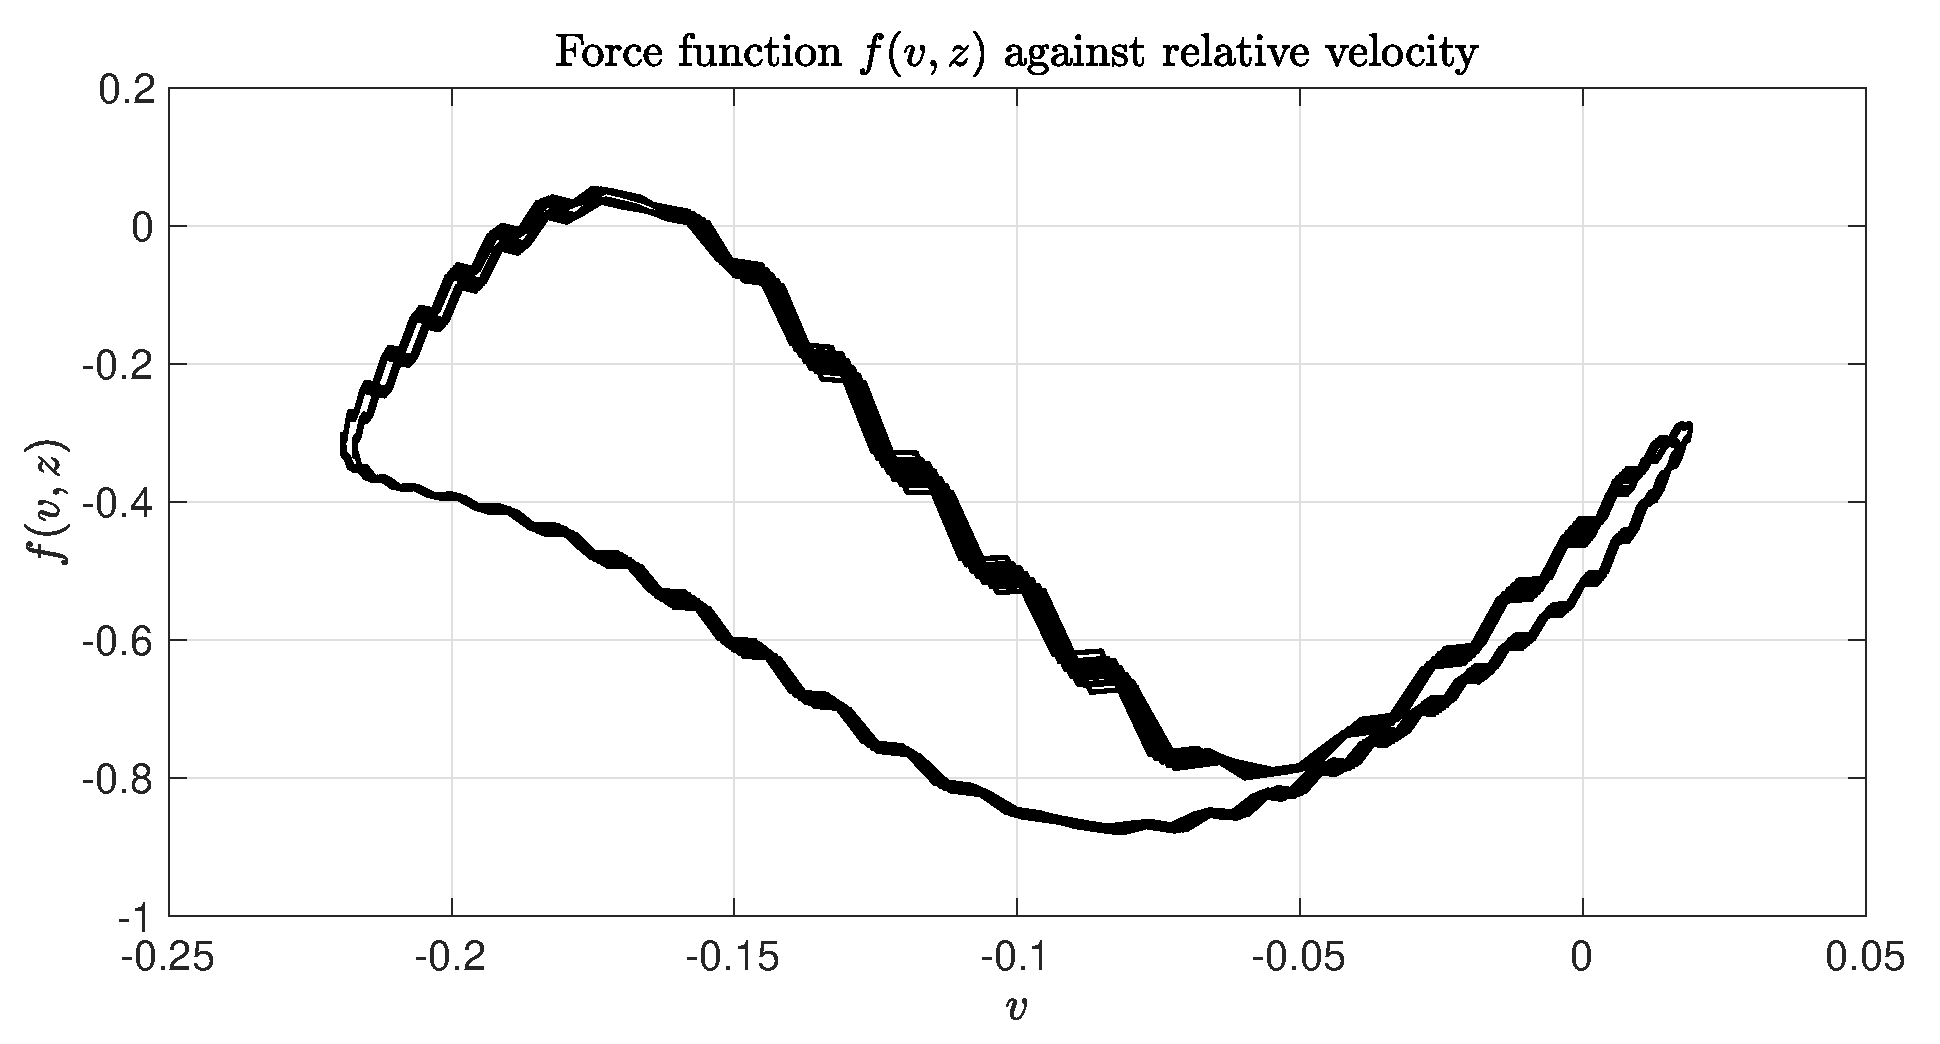
\includegraphics[width=1.0\columnwidth]{hysteresis.eps}}
\caption{\label{fig:hysteresis}Hysteresis loop.}
\end{figure}


$<5\%$ CPU usage. 
\section{Conclusions}\label{sec:conclusion}
This template can be found on the conference website.
For changing the number of author affiliations (1 to 4), uncomment the corresponding regions in the template \texttt{tex} file.
Please, submit full-length papers (max.~8 pages both oral and poster presentations).
Submission is fully electronic and automated through the Conference Web Submission System.
DO NOT send us papers directly by e-mail.

\section{Acknowledgments}
Many thanks to the great number of anonymous reviewers!

%\newpage
\nocite{*}
\bibliographystyle{IEEEbib}
\bibliography{DAFx19_tmpl} % requires file DAFx19_tmpl.bib

\section{Appendix: Interpolation and Spreading Operators}
\label{app:interpol}
In this section, the interpolator and spreading operator introduced in Section \ref{sec:discretisation} will be explained.

The simplest way to select a grid point $l_\text{B}$ from bowing position $x_\text{B}$ on a discrete string is $l_\text{B} = \text{floor}(x_\text{B}/h)$. Applied to a gridfunction $u_l$ yields
\begin{equation}
    I_0(x_\text{B})u_l = u_{l_\text{B}}.
\end{equation}
More accurate would be to use linear interpolation 
\begin{equation}\label{eq:linearInterpolation}
     I_1(x_\text{B})u_l =
      (1-\alpha_\text{B})u_{l_\text{B}}+ \alpha_\text{B}u_{l_\text{B}+1}
\end{equation}
where $\alpha_\text{B} = x_\text{B}/h - l_\text{B}$ is the fractional remainder of the flooring operation. Even more accurate would be to use cubic interpolation:
% \begin{equation}\label{eq:cubicInterpolation}
% \begin{aligned}
%      I_3(x_\text{B})u_{l_\text{B}} =&  \frac{\alpha_\text{B}(\alpha_\text{B}-1)(\alpha_\text{B} - 2)}{-6}u_{l_\text{B}-1}+\\
%      &\frac{(\alpha_\text{B}-1)(\alpha_\text{B}+1)(\alpha_\text{B}-2)}{2}u_{l_\text{B}}+  \frac{\alpha_\text{B}(\alpha_\text{B}+1)(\alpha_\text{B} - 2)}{-2}u_{l_\text{B}+1} \\
%      &+ \frac{\alpha_\text{B}(\alpha_\text{B}+1)(\alpha_\text{B} - 1)}{6}u_{l_\text{B}+2}
%      \end{aligned}
% \end{equation}
\begin{equation}
I_3(x_\text{B}) =
     \begin{cases}
    \hfil 0, & l < l_{\text{B}} - 1\\
    \hfil \alpha_\text{B}(\alpha_\text{B}-1)(\alpha_\text{B} - 2)/{-6}, & l = l_{\text{B}} - 1\\
    \hfil (\alpha_\text{B}-1)(\alpha_\text{B}+1)(\alpha_\text{B}-2)/2, & l = l_{\text{B}}\\
    \hfil \alpha_\text{B}(\alpha_\text{B}+1)(\alpha_\text{B} - 2)/{-2}, & l = l_{\text{B}} + 1\\
    \hfil \alpha_\text{B}(\alpha_\text{B}+1)(\alpha_\text{B} - 1)/6, & l = l_{\text{B}} +2,\\
    \hfil 0, & l > l_\text{B} + 2
    \end{cases}
    \end{equation}
spreading operator $J$ can be defined as linear \cite{Bilbao2009}:
\begin{equation}\label{eq:linearSpreading}
     J_1(x_\text{B}) = \frac{1}{h}
     \begin{cases}
    \hfil 0, & l < l_{\text{B}}\\
    \hfil (1-\alpha_\text{B}), & l = l_{\text{B}}\\
    \hfil \alpha_\text{B}, & l = l_{\text{B}} + 1\\
    \hfil 0, & l > l_\text{B} + 1
\end{cases}
\end{equation}
or cubic:
\begin{equation}\label{eq:cubicInterpolation}
     J_3(x_\text{B}) = \frac{1}{h}
     \begin{cases}
    \hfil 0, & l < l_{\text{B}} - 1\\
    \hfil \alpha_\text{B}(\alpha_\text{B}-1)(\alpha_\text{B} - 2)/{-6}, & l = l_{\text{B}} - 1\\
    \hfil (\alpha_\text{B}-1)(\alpha_\text{B}+1)(\alpha_\text{B}-2)/2, & l = l_{\text{B}}\\
    \hfil \alpha_\text{B}(\alpha_\text{B}+1)(\alpha_\text{B} - 2)/{-2}, & l = l_{\text{B}} + 1\\
    \hfil \alpha_\text{B}(\alpha_\text{B}+1)(\alpha_\text{B} - 1)/6, & l = l_{\text{B}} +2,\\
    \hfil 0, & l > l_\text{B} + 2
\end{cases}
\end{equation}
\end{document}
